\section{Descripción del problema}
\label{desc_problem}

En esta sección se expondrá la descripción del problema a resolver en el marco de esta tesina: para ello, en primer lugar, se presentará el fundamento teórico básico detrás de una huella digital; posteriormente se harán observaciones sobre las dificultades de controlar estas huellas digitales de manera centralizada. Luego de este punto, se brindará una breve reseña histórica sobre la descentralización de los sistemas y el potencial de este tipo de arquitecturas. Finalmente, se cerrará el capítulo con una reflexión, preparando el terreno para ahondar en el marco teórico.

\subsection{Problema de la integridad de datos}

Desde el surgimiento de Internet en 1990 y el advenimiento de la descarga de archivos a través de esta red, siempre ha sido un problema garantizar la integridad de los mismos, es decir, poder probar mediante un método riguroso que estos no son alterados en ningún momento. Estas potenciales modificaciones pueden ser aleatorias, por ejemplo, debido a fallas del medio de transmisión, o bien, porque un agente malintencionado introduce un cambio indebido.

\subsection{Funciones de una sola vía}
\label{funcion_una_sola_via}

Dentro del marco de Internet, uno de los primeros algoritmos utilizados para verificar la integridad de los archivos transferidos fue MD5 \cite{Rivest1992}, el cual pertenece a la familia de funciones de \textit{hash} una sola vía (\textit{one-way function}). Este tipo de funciones tiene como objetivo asociar cada elemento del dominio que, en el presente caso, está caracterizado por el conjunto de archivos posibles (el cual es infinito) con una cadena pseudo-aleatoria y fija de caracteres. Matemáticamente, podría modelarse de la siguiente manera:

\begin{equation}
  f_k(a) = m_k
\end{equation}

Donde $f_k$ es la función que se aplica sobre el archivo $a$ y genera una cadena $m_k$ de longitud $k$. Esta cadena representa la \textit{huella digital} de tal archivo.
La particularidad de las funciones de una sola vía es que el costo computacional que se invierte para obtener el valor $m_k$ a partir de $a$ es muy barato, mientras que el proceso inverso, es decir, el recuperar el archivo $a$ a partir de la huella $m_k$ es virtualmente imposible. Esta característica las hace especialmente idóneas para la verificación de integridad de archivos sobre redes de datos: genéricamente, si en un nodo cualquiera de la red se computa el valor $f_k(a)$ y se deja accesible de forma pública, entonces cualquier otro nodo de la misma red podría corroborar que el archivo $a$ transferido fue recibido de forma intacta computando la misma función sobre dicho archivo, y luego, verificando que el resultado sea igual a la \textit{huella} generada por el nodo origen; de lo contrario, se inferirá que hubo algún tipo de alteración sobre él.

\subsection{Problemas inherentes}

Una de las cuestiones a considerar muy cuidadosamente cuando se diseña un algoritmo o una función de una sola vía es evitar las colisiones. Una colisión es un fenómeno en el cual el valor computado de la función para dos objetos (archivos) distintos es exactamente el mismo. Formalmente:

\begin{equation}
  f_k(a) = f_k(b), \quad a \neq b
\end{equation}

Si esta situación ocurre y, además, se comprende desde la lógica del algoritmo cómo y por qué ocurre entonces a partir de esto sería relativamente sencillo fraguar o deliberadamente alterar archivos con el propósito de que posea la misma huella digital que otro archivo y que contenga otra información potencialmente dañina.

Por ejemplo, volviendo al caso particular de MD5, en el año 2005 \cite{wang2005break} se constató que dicha función presentaba colisiones de forma sistémica, con lo cual, se fue dejando de emplear para computar huellas digitales.

\subsection{Problemas de centralización}

Aun en el caso de disponer de una función de una sola vía relativamente segura, muchas veces el mayor problema recae en la arquitectura, particularmente, aquellas en la que la seguridad se concentra en un único punto o servidor.

Además de los problemas de rendimiento conocidos, en donde un número reducido de servidores podría colapsar ante una gran cantidad de peticiones por parte de los usuarios o clientes \cite{NeilsonWoodside1995}, existen también problemas de seguridad asociados. Si, por ejemplo, un atacante consigue tomar control del/los servidor/es del sistema, entonces cualquier información alojada en ella dejaría de ser automáticamente confiable, en particular, las huellas digitales publicadas de los archivos ubicados allí. Al administrar el servidor, un agente malintencionado podría cambiar los archivos, recomputar sus huellas y republicarlas al exterior y todo el circuito parecería confiable, pero sin embargo, el agente ha conseguido romper un eslabón de confiabilidad y eso podría ser muy costoso para el proceso o negocio involucrado.

\subsection{Arquitecturas descentralizadas}

Dadas las problemáticas de las redes centralizadas basadas en arquitecturas cliente-servidor, una variante desarrollada en pos de mitigar este inconveniente fue pensar las redes sin la noción típica de ``servidor central'', sino más bien, pensar en redes donde cada nodo participante de ella pueda requerir información o trabajo como así también suministrar información o trabajo. Cabe destacar que hay distintos niveles de descentralización; por ejemplo, lo que se describió previamente es una instancia de red descentralizada pura dado que todos los nodos actúan como clientes y servidores a la vez. Sin embargo, esto no necesariamente se da así en la realidad. En otros casos la red puede ser mixta, esto es, una red con un número equilibrado y bien distribuido -ya sea lógica o físicamente- de servidores y clientes.

En la figura \ref{fig:topologia-tipo-redes} se muestra una comparación topológica básica de estos dos tipos de redes.

\begin{figure}[H]
  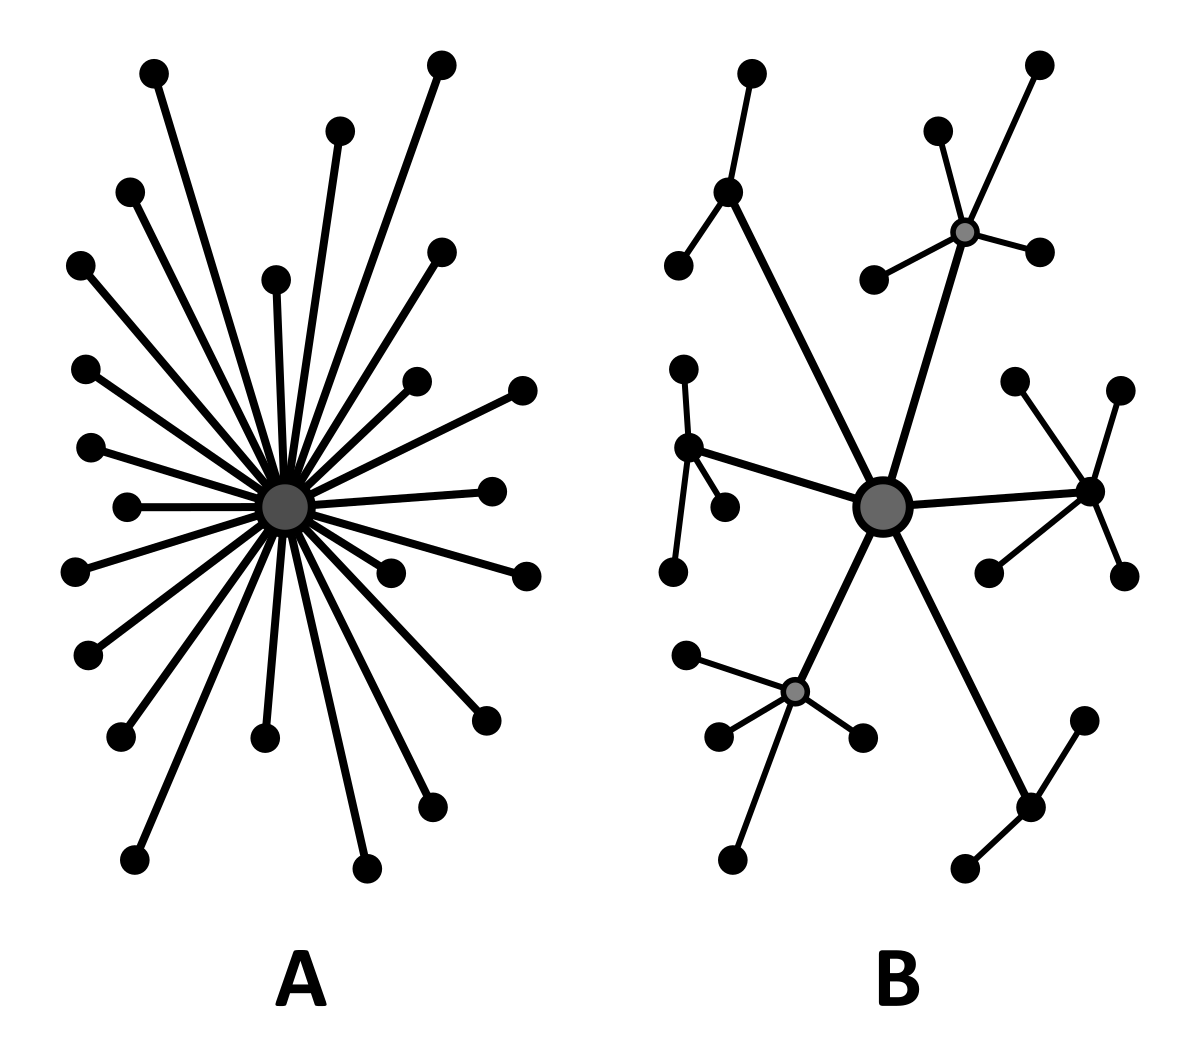
\includegraphics[height=8cm, width=8cm]{decentralization_diagram.png}
  \centering
  \caption{Topología de los distintos tipos de redes}
  \label{fig:topologia-tipo-redes}
\end{figure}

El gráfico A muestra un ejemplo de red totalmente centralizado en donde un solo nodo coordina o abastece el trabajo del resto de los participantes. En este caso, se puede notar claramente que si ese único nodo falla o, peor aún, es saboteado por un agente maligno, consecuentemente toda la red caerá o será controlada por dicho nodo central bajo potenciales efectos dañinos.

Por otro lado, el gráfico B muestra una arquitectura descentralizada mixta compuesta por varios cúmulos o \textit{clusters}. Si uno de los nodos responsables del control de un cúmulo es abordado malintencionadamente, el mismo se mantendrá fuera de control, pero dicha acción no afectará el curso total de la red.

Esta última característica es crucial para el presente trabajo puesto que la confianza ahora no dependerá solamente de un único punto sino de muchos otros, y esto, como se analizará posteriormente, disminuye exponencialmente la probabilidad de obtener todo el control de la red con el objeto de anunciar información espuria sobre ella.

\subsubsection{Historia de la descentralización}
\label{historia_descentralizacion}

Una de las primeras personas en investigar y proponer casos de uso concretos basándose en las ideas y las virtudes de la descentralización fue David Lee Chaum. En el año 1981 publicó un trabajo llamado \textit{Untraceable Electronic Mail, Return Addresses, and Digital Pseudonyms}\cite{Chaum1981} donde se brinda una solución al \textit{Problema del análisis de tráfico} el cual consiste en ocultar quién se comunica con quién y cuándo. Si bien en la época se habían desarrollado soluciones para este problema, la descrita en el trabajo de Chaum fue la primera en hacerlo de manera totalmente descentralizada, es decir, sin contar con los riesgos de tener que confiar en una autoridad central. Para ello, propone el uso de una red denominada \textit{Mix Network} en donde todos los nodos participantes son responsables de encriptar y desencriptar los mensajes en lotes paso a paso. El atractivo principal de este tipo de arquitectura para este problema es que si alguien con propósitos malévolos toma ilegítimamente el control de uno de los nodos (o incluso de varios), la red puede seguir garantizando su funcionamiento y su confiabilidad; en cambio, en una arquitectura con una autoridad central, cuando esta última es atacada y capturada, la confianza y la seguridad de toda la red queda totalmente comprometida porque el cumplimiento de estas propiedades depende precisamente de este nodo central.

En 1982 Chaum presentó su tesis doctoral titulada \textit{Computer Systems Established, Mantained and Trusted by Mutually Suspicius Group}\cite{Chaum1982} en donde se discute y se especifica formalmente la factibilidad y el diseño de un sistema genérico sobre el cual un conjunto de organizaciones no emparentadas entre si, es decir, sin requisitos de confianza mutua, puedan trabajar de forma segura y fiable mediante una ``caja fuerte'' (\textit{vault}). En dicho trabajo se explora exhaustivamente las técnicas de criptografía de clave pública, y respecto a la ``caja fuerte'', se demuestran las ventajas de disponer de muchas de ellas como forma de evitar el problema del único punto de falla.

En 1983 Chaum dio a conocer un nuevo artículo denominado \textit{Blind Signatures for Untraceable Payments}\cite{Chaum1983} en el cual se aborda específicamente, y por primera vez, la forma de realizar pagos -o transacciones de bienes- de manera anónima y segura. Se desarrolla para ello el concepto de firmas ciegas para disponer de autenticidad, trazabilidad y, al mismo tiempo, confidencialidad sobre los movimientos efectuados. Si bien este sistema propuesto no aborda la descentralización de las operaciones, en el mismo trabajo se menciona que dicha posibilidad podría ser plausible (tal como se demuestra en \cite{Chaum1982}) y se deja el terreno preparado para la introducción de un sistema transaccional completamente descentralizado.

\subsection{Recapitulación}
\label{recapitulacion_desc_problema}

En esta sección se ha presentado la idea de ``huella digital'' para archivos utilizando como herramienta matemática para tal fin a las funciones de una sola vía; se ha descrito el problema a tratar en este trabajo en donde no es conveniente publicar y gestionar dichas huellas en un servidor centralizado para evitar que la confiabilidad y la seguridad recaiga en único punto dentro de la arquitectura. A través de los distintos trabajos revelados a lo largo de la historia -y enunciados en este informe- se ha podido visualizar que la problemática de centralizar la información o, de manera equivalente, que la misma sea controlada por una autoridad central fue un punto a evitar y, consecuentemente, se han propuestos alternativas conceptuales -a nivel arquitectónico fundamentalmente- para eludir la cuestión del ``único punto de falla'' y obtener el control de todo un sistema por dicho medio.

Se puede establecer, como para concluir esta sección, que el uso de una arquitectura descentralizada robusta podría ofrecer claras ventajas, con miras a la fiabilidad y a la transparencia de las operaciones, respecto a una clásica arquitectura de un sólo servidor y muchos clientes para el problema que se ha planteado.
